\chapter{Fundamentals \textRoman{3}: Band Topology}
\label{cha:fundamentals_c}

% opening paragraph
We continue our discussion of the fundamentals in this chapter, where we introduce the topology of electronic bands.
Chapter~\ref{cha:fundamentals_a} established the electronic states and their energies within the Kohn--Sham framework.
Chapter~\ref{cha:fundamentals_b} then connected these states to the optical response through transition matrix elements and energy differences.
We now examine another property of the same electronic states:
how they can be connected continuously across the Brillouin zone while preserving the symmetries of the system.
This connection contains information that is not specified by the band energies alone.

The discussion follows the parity analysis used for the beryllene systems in chapter~\ref{cha:project_beryllene}.
We first recover the Bloch states and identify the band subspace to which a topological index can be assigned.
We then introduce phase freedom and the Berry phase to explain why comparing electronic states requires more than comparing their energies.
Next, we consider time-reversal and inversion symmetry, which determine the pairing and parity of the spinor states.
Finally, we use these properties to obtain the two-dimensional $Z_2$ index from the Fu--Kane parity criterion.
Throughout this discussion, we distinguish the topology of a selected band subspace from an insulating state at the Fermi level.
This distinction is required when interpreting the metallic systems considered in the present work.

\newpage
\section{Toward the topology of Bloch states}
\label{sec:toward_band_topology}

% opening paragraph
In the previous two chapters, the electronic states entered two different questions.
For the ground-state problem, we determined the states that reproduce the electron density.
For the optical problem, we examined how an external field induces transitions between these states.
The topological problem instead compares states at different wave vectors.
Before making this comparison, we therefore need to identify both the states and the subspace that they form.

\subsection{From band energies to electronic states}

We begin with the Bloch representation introduced in equation~\eqref{bloch_state_cell_periodic_method}.
For a periodic one-particle hamiltonian $\hat{h}$, we write:

\begin{equation}
\left\{\begin{aligned}
    \ket{\psi_{n\vec{k}}}
    &=\mathrm{e}^{\mathrm{i}\vec{k}\cdot\hat{\vec{r}}}\ket{u_{n\vec{k}}} \\
    \hat{h}(\vec{k})
    &\coloneqq\mathrm{e}^{-\mathrm{i}\vec{k}\cdot\hat{\vec{r}}}
    \hat{h}\,\mathrm{e}^{\mathrm{i}\vec{k}\cdot\hat{\vec{r}}} \\
    \hat{h}(\vec{k})\ket{u_{n\vec{k}}}
    &=E_{n\vec{k}}\ket{u_{n\vec{k}}}
\end{aligned}\right.
\label{bloch_hamiltonian_topology}
\end{equation}

here, $n$ denotes the band index, $\vec{k}$ denotes the crystal wave vector,
and $\hat{\vec{r}}$ is the position operator.
The state $\ket{u_{n\vec{k}}}$ is the cell-periodic part of the Bloch state,
normalized over one unit cell as in chapter~\ref{cha:fundamentals_a}.
In this chapter, inner products between cell-periodic states use this cell normalization.
The operator $\hat{h}$ denotes the effective electronic hamiltonian,
including spin-orbit coupling when we consider the spinful topological classification below.

The eigenvalues $E_{n\vec{k}}$ provide the band dispersion.
However, the eigenvalue equation also provides an electronic state at each $\vec{k}$.
Two neighbouring points in the Brillouin zone therefore carry not only two sets of energies,
but also two sets of states that can be compared through their overlaps.
As we move through the Brillouin zone, these overlaps describe how the electronic states change.
Band topology concerns the global structure of this connection.

There is already a freedom in specifying an individual normalized state.
For any real phase $\phi_n(\vec{k})$, we can replace it by:

\begin{equation}
    \ket{u'_{n\vec{k}}}
    =\mathrm{e}^{\mathrm{i}\phi_n(\vec{k})}\ket{u_{n\vec{k}}}
\label{bloch_phase_freedom_topology}
\end{equation}

This replacement changes neither the band energy nor the projector
$\ket{u_{n\vec{k}}}\bra{u_{n\vec{k}}}$.
It therefore represents the same physical state.
However, a derivative with respect to $\vec{k}$ also differentiates the chosen phase.
Consequently, we must account for this freedom when connecting states at different wave vectors.
We return to this point after identifying the band subspace of interest.

\subsection{An isolated band subspace}
\label{subsec:isolated_band_subspace_topology}

For the spinful, time-reversal-symmetric systems considered below,
we select the lowest $2N_\mathrm{p}$ bands at every $\vec{k}$,
where $N_\mathrm{p}$ denotes the number of Kramers pairs at a time-reversal invariant momentum.
We order the band energies increasingly, counting each spinor state once.
The projector onto the selected subspace is then:

\begin{equation}
    \hat{\mathcal{P}}(\vec{k})
    \coloneqq\sum_{n=1}^{2N_\mathrm{p}}
    \ket{u_{n\vec{k}}}\bra{u_{n\vec{k}}}
\label{band_subspace_projector_topology}
\end{equation}

here, the rank $2N_\mathrm{p}$ is fixed throughout the Brillouin zone.
The projector specifies which states belong to the subspace,
without selecting a particular basis within it.
This distinction becomes useful when bands inside the selected subspace cross or become degenerate.
An individual eigenstate may then be difficult to follow continuously,
although the subspace formed by all the selected states remains well defined.

To separate this subspace from the remaining bands,
we require a positive direct separation at every wave vector:

\begin{equation}
\left\{\begin{aligned}
    \Delta_\mathrm{dir}(\vec{k})
    &\coloneqq E_{2N_\mathrm{p}+1,\vec{k}}-E_{2N_\mathrm{p},\vec{k}} \\
    \Delta_\mathrm{dir}^\mathrm{min}
    &\coloneqq\min_{\vec{k}\in\mathrm{BZ}}\Delta_\mathrm{dir}(\vec{k})>0
\end{aligned}\right.
\label{minimum_direct_gap_topology}
\end{equation}

This is the separation introduced in equation~\eqref{isolated_band_subspace_method}.
The condition concerns the boundary between the selected and excluded bands.
Degeneracies wholly inside the selected subspace do not close this separation.
For a smooth periodic hamiltonian, the separation allows the spectral projector
$\hat{\mathcal{P}}(\vec{k})$ to vary smoothly across the Brillouin zone.
The choice of basis for that projector may still require different local phase conventions.

We next ask whether the same condition also makes the system insulating.
The direct separation compares two energies at the same $\vec{k}$.
An insulating gap instead requires the highest energy of the selected bands to lie below the lowest energy of the excluded bands,
even when these energies occur at different wave vectors.
We therefore define the global, or indirect, separation as:

\begin{equation}
    \Delta_\mathrm{ind}
    \coloneqq\min_{\vec{k}\in\mathrm{BZ}}E_{2N_\mathrm{p}+1,\vec{k}}
    -\max_{\vec{k}\in\mathrm{BZ}}E_{2N_\mathrm{p},\vec{k}}
\label{indirect_gap_topology}
\end{equation}

For $\Delta_\mathrm{ind}>0$, there is an energy interval separating the two sets of bands.
If the electron filling places the Fermi energy in this interval,
the selected subspace is the occupied subspace of a band insulator.
At zero temperature, this requires:

\begin{equation}
    \max_{\vec{k}\in\mathrm{BZ}}E_{2N_\mathrm{p},\vec{k}}
    <E_\mathrm{F}
    <\min_{\vec{k}\in\mathrm{BZ}}E_{2N_\mathrm{p}+1,\vec{k}}
\label{insulating_fermi_level_topology}
\end{equation}

In contrast, $\Delta_\mathrm{dir}^\mathrm{min}>0$ can coexist with $\Delta_\mathrm{ind}<0$.
The selected subspace then remains separated at every individual $\vec{k}$,
while its energy range overlaps that of the excluded bands.
At the corresponding filling, this overlap can produce electron and hole pockets.
The states below $E_\mathrm{F}$ are consequently not the same fixed-rank subspace at every wave vector.
We must therefore specify the band count when assigning a topological index to such a subspace.

\begin{figure}[htbp]
\centering
    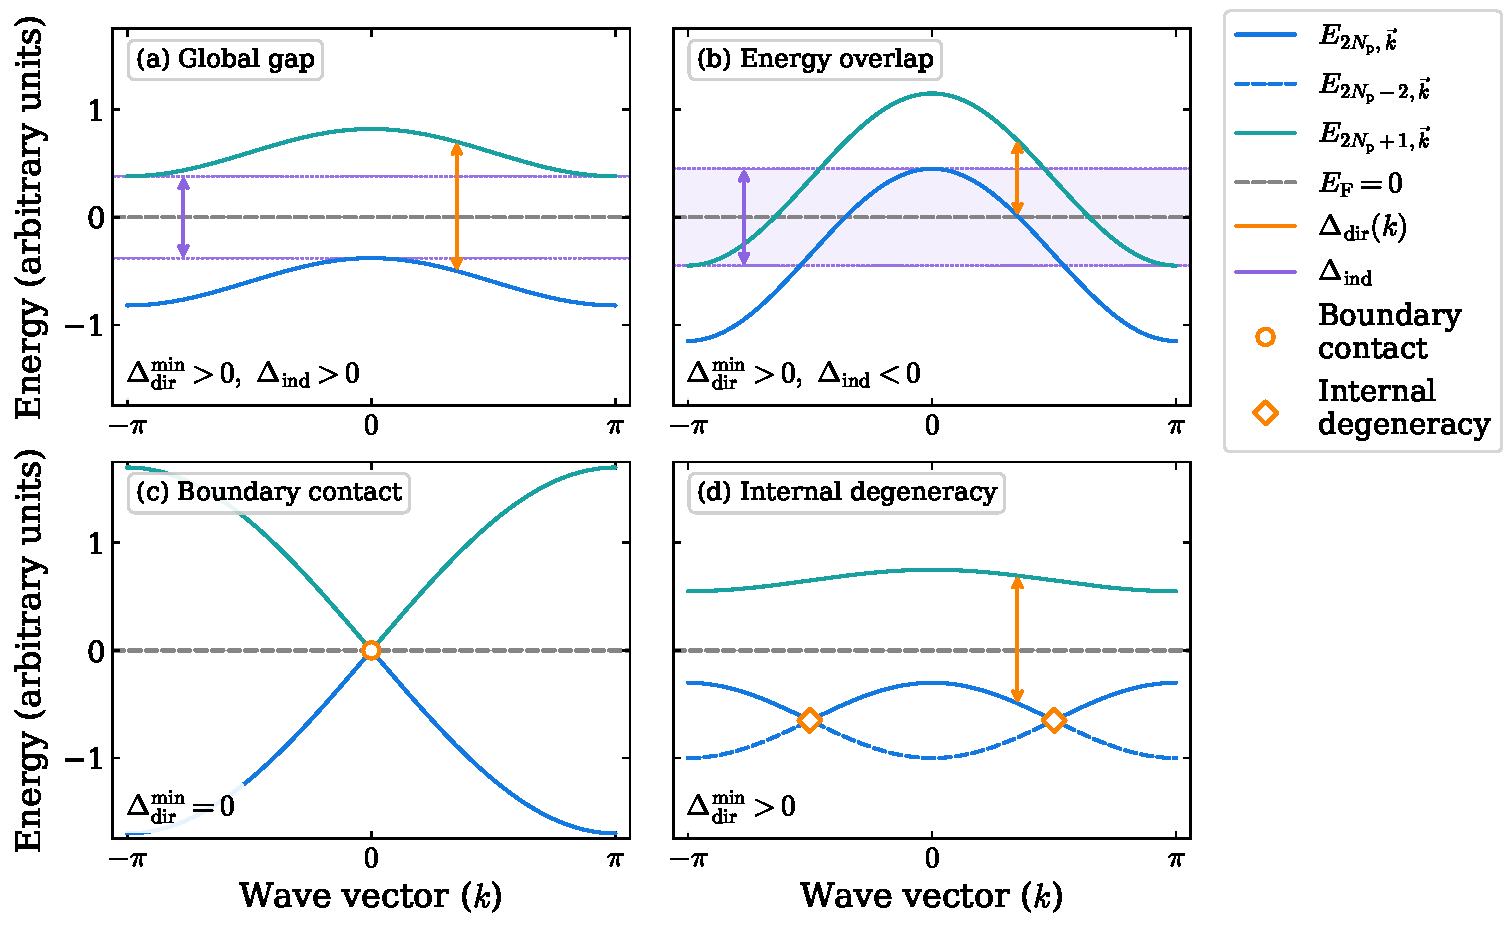
\includegraphics[width=0.95\textwidth]{figures_ch4/4.1_band_subspace.pdf}
\caption{Schematic distinction between an isolated band subspace and an insulating gap.
The blue and teal curves represent the boundary bands $E_{2N_\mathrm{p},\vec{k}}$ and $E_{2N_\mathrm{p}+1,\vec{k}}$, respectively.
(a) Positive direct and indirect gaps permit an insulating filling.
(b) The direct separation remains positive despite an indirect energy overlap, shaded in purple.
(c) A band touching closes the separation of the selected subspace.
Orange arrows compare energies at the same wave vector; purple arrows and dotted extrema indicate the indirect separation.
The grey dashed line denotes the illustrative Fermi level $E_\mathrm{F}=0$.
The model dispersions use arbitrary energy units and a dimensionless periodic coordinate $k$.
They are schematic one-dimensional cuts, not calculated beryllene bands; isolation over the full two-dimensional Brillouin zone requires a separate check.}
\label{fig:band_subspace_and_insulating_gap}
\end{figure}

Figure~\ref{fig:band_subspace_and_insulating_gap} separates these three situations.
The first two permit a smooth fixed-rank projector, provided the direct separation holds over the full Brillouin zone.
The third loses the spectral separation at the boundary of the chosen subspace.
We can now discuss how the states within an isolated subspace are connected,
while keeping the separate question of the physical Fermi level explicit.

\newpage
\section{From phase freedom to the Berry phase}
\label{sec:berry_phase_topology}

% opening paragraph
The previous section identified the electronic subspace and the condition that separates it from the remaining bands.
We now examine the connection between states at neighbouring wave vectors.
The phase freedom in equation~\eqref{bloch_phase_freedom_topology} means that an individual overlap depends on how the states are represented.
A closed sequence of overlaps, however, can retain information that is independent of those local phase choices.
This provides the geometric starting point for discussing band topology.

\subsection{Connecting neighbouring states}

We first consider a single normalized band that is non-degenerate along a path.
This simpler case allows us to identify the phase information before returning to a group of bands.
For a small displacement $\dif\vec{k}$, the overlap between neighbouring cell-periodic states is:

\begin{equation}
    \braket{u_{n\vec{k}}|u_{n,\vec{k}+\dif\vec{k}}}
    =1+
    \bra{u_{n\vec{k}}}\nabla_{\vec{k}}\ket{u_{n\vec{k}}}
    \cdot\dif\vec{k}
    +\mathcal{O}(|\dif\vec{k}|^2)
\label{neighbouring_bloch_overlap_topology}
\end{equation}

Normalization requires the real part of
$\bra{u_{n\vec{k}}}\nabla_{\vec{k}}\ket{u_{n\vec{k}}}$ to vanish.
The first-order change of the overlap therefore carries a phase.
We describe this phase variation by introducing the Berry connection~\cite{berry1984quantal}:

\begin{equation}
    \vec{\mathcal{A}}_n(\vec{k})
    \coloneqq\mathrm{i}\,
    \bra{u_{n\vec{k}}}\nabla_{\vec{k}}\ket{u_{n\vec{k}}}
\label{berry_connection_topology}
\end{equation}

here, $\nabla_{\vec{k}}$ differentiates the cell-periodic state with respect to the wave vector.
With $\vec{k}$ measured in inverse length, $\vec{\mathcal{A}}_n$ has the dimension of length,
and $\vec{\mathcal{A}}_n\cdot\dif\vec{k}$ is dimensionless.
Equation~\eqref{neighbouring_bloch_overlap_topology} consequently takes the form
$1-\mathrm{i}\,\vec{\mathcal{A}}_n\cdot\dif\vec{k}$ to first order.

We next substitute the phase transformation in equation~\eqref{bloch_phase_freedom_topology} into this definition.
Differentiating both the phase factor and the state gives:

\begin{equation}
    \vec{\mathcal{A}}'_n(\vec{k})
    =\vec{\mathcal{A}}_n(\vec{k})-\nabla_{\vec{k}}\phi_n(\vec{k})
\label{berry_connection_gauge_transformation_topology}
\end{equation}

The Berry connection therefore depends on the phase convention, also called the gauge.
This dependence follows directly from our freedom to choose a representative for the same physical state.
We must close the path before identifying a phase that is independent of the arbitrary choices at individual points.

\subsection{Closing the path}

Let $C$ be an oriented closed path on which the band remains non-degenerate.
For a smooth gauge that is single-valued around this path, the Berry phase is:

\begin{equation}
    \gamma_n(C)
    =\oint_C\vec{\mathcal{A}}_n(\vec{k})\cdot\dif\vec{k}
    \qquad (\mathrm{mod}\ 2\pi)
\label{berry_phase_closed_path_topology}
\end{equation}

Under equation~\eqref{berry_connection_gauge_transformation_topology},
the change in $\gamma_n(C)$ is the negative of the phase change accumulated around the loop.
For a single-valued gauge transformation, this change is an integer multiple of $2\pi$.
Thus $\mathrm{e}^{\mathrm{i}\gamma_n(C)}$ is unchanged.
The local phase choices cancel, while the phase accumulated by connecting the states around the loop remains.

The same cancellation can be seen by discretizing the path into $M$ points.
With the endpoint identified with the starting point, we write:

\begin{equation}
    \gamma_n(C)
    =-\lim_{M\rightarrow\infty}\arg
    \prod_{j=0}^{M-1}
    \braket{u_{n\vec{k}_j}|u_{n\vec{k}_{j+1}}}
    \qquad (\mathrm{mod}\ 2\pi)
\label{berry_phase_overlap_product_topology}
\end{equation}

here, the endpoint state is identified consistently with the initial state,
including the reciprocal-lattice transformation if the loop crosses a Brillouin-zone boundary.
The mesh must be fine enough that successive overlaps are non-zero.
Every local phase then appears once in a bra and once in a ket, so it cancels from the product.
The minus sign follows from the convention in equation~\eqref{berry_connection_topology}.

The Berry phase describes the geometry of the electronic states along a chosen loop.
It is not generally restricted to $0$ or $\pi$,
and a Berry phase on an arbitrary loop is not by itself the two-dimensional $Z_2$ index.
The additional structure needed for that index comes from time-reversal symmetry and the full selected band subspace.

\subsection{From an individual band to a band subspace}

The single-band discussion assumes that the state can be followed separately from all other states along the path.
For spinful time-reversal-symmetric systems, degeneracies are instead part of the problem.
We therefore return to the projector in equation~\eqref{band_subspace_projector_topology}.

Within its $2N_\mathrm{p}$-dimensional subspace, we may choose a different orthonormal basis:

\begin{equation}
\left\{\begin{aligned}
    \ket{u'_{a\vec{k}}}
    &=\sum_{n=1}^{2N_\mathrm{p}}
    \ket{u_{n\vec{k}}}U_{na}(\vec{k}) \\
    U^\dagger(\vec{k})U(\vec{k})&=I \\
    \sum_{a=1}^{2N_\mathrm{p}}\ket{u'_{a\vec{k}}}\bra{u'_{a\vec{k}}}
    &=\hat{\mathcal{P}}(\vec{k})
\end{aligned}\right.
\label{band_subspace_basis_transformation_topology}
\end{equation}

here, $U(\vec{k})$ is a unitary matrix and $I$ is the identity matrix within the selected subspace.
The transformed basis need not diagonalize the hamiltonian when it mixes states of different energies.
Nevertheless, it describes the same projector and therefore the same band subspace.
This is the multi-state counterpart of the phase freedom introduced earlier.

For such a basis, the connection becomes a matrix~\cite{wilczek1984appearance}.
Applying the same derivative as in equation~\eqref{berry_connection_topology} to each pair of basis states gives:

\begin{equation}
\left\{\begin{aligned}
    [\vec{\mathcal{A}}(\vec{k})]_{mn}
    &=\mathrm{i}\bra{u_{m\vec{k}}}\nabla_{\vec{k}}\ket{u_{n\vec{k}}} \\
    \vec{\mathcal{A}}'(\vec{k})
    &=U^\dagger(\vec{k})\vec{\mathcal{A}}(\vec{k})U(\vec{k})
    +\mathrm{i}\,U^\dagger(\vec{k})\nabla_{\vec{k}}U(\vec{k})
\end{aligned}\right.
\label{band_subspace_connection_topology}
\end{equation}

here, $m$ and $n$ run over the selected basis states.
The second relation follows by differentiating both the original basis and the matrix $U(\vec{k})$.
For a single state, it reduces to equation~\eqref{berry_connection_gauge_transformation_topology}.
The off-diagonal elements describe the mixing of basis states as $\vec{k}$ changes.
Consequently, assigning independent single-band phases to arbitrary members of a degenerate pair does not characterize the whole subspace.
In the present work, inversion symmetry provides a way to determine the required $Z_2$ index directly from parity eigenvalues.
Before introducing that criterion, we need to establish how time reversal and inversion act on the same states.

\newpage
\section{Time-reversal and inversion symmetry}
\label{sec:symmetry_and_kramers_pairs_topology}

% opening paragraph
The previous section showed why the phase convention of an individual state cannot determine the topology of a band subspace.
We now impose the symmetries relevant to the beryllene parity analysis.
Time reversal connects states at opposite wave vectors and determines their Kramers pairing.
Inversion also reverses the wave vector, while assigning a parity at the momenta where the state returns to the same crystal momentum.
Together, these two symmetries provide the information used in the parity criterion.

\subsection{Spinor states and time reversal}

With spin-orbit coupling, the spatial and spin parts of an electronic state need not separate.
Following equation~\eqref{KS_spinor_equation_method}, we express the cell-periodic state as:

\begin{equation}
    \ket{u_{n\vec{k}}}
    =\ket{u_{n\vec{k},\uparrow}}\otimes\ket{\uparrow}
    +\ket{u_{n\vec{k},\downarrow}}\otimes\ket{\downarrow}
\label{cell_periodic_spinor_topology}
\end{equation}

here, the two spatial components form one spinor state.
They are not two separate occupied bands.
Spin-orbit coupling can mix these components, so spin is not generally a conserved band label.
The time-reversal classification, however, remains applicable when the hamiltonian preserves time-reversal symmetry.

For spin-$1/2$ electrons, we choose the time-reversal operator as:

\begin{equation}
\left\{\begin{aligned}
    \hat{\Theta}&=\mathrm{i}\hat{\sigma}_y\hat{K} \\
    \hat{\Theta}^2&=-\hat{I} \\
    \hat{\Theta}\hat{h}(\vec{k})\hat{\Theta}^{-1}
    &=\hat{h}(-\vec{k})
\end{aligned}\right.
\label{spinful_time_reversal_topology}
\end{equation}

here, $\hat{\sigma}_y$ is the Pauli operator in the chosen spin basis,
$\hat{K}$ takes the complex conjugate in the position and spin representation,
and $\hat{I}$ is the identity operator.
The last relation states the symmetry condition on the hamiltonian.
It applies to the non-magnetic spinful problem considered here;
spin-orbit coupling alone does not break time-reversal symmetry.

The operator $\hat{\Theta}$ is antiunitary.
For any two states, it therefore satisfies
$\braket{\hat{\Theta}a|\hat{\Theta}b}=\braket{b|a}$.
To apply this relation at a TRIM, we use a full Bloch state $\ket{\psi}$,
so equivalent crystal momenta belong to the same translation sector.
Taking $\ket{a}=\ket{\psi}$ and $\ket{b}=\hat{\Theta}\ket{\psi}$ gives:

\begin{equation}
    \braket{\hat{\Theta}\psi|\psi}
    =\braket{\hat{\Theta}\psi|\hat{\Theta}^2\psi}
    =-\braket{\hat{\Theta}\psi|\psi}
\label{kramers_orthogonality_topology}
\end{equation}

Consequently, $\braket{\hat{\Theta}\psi|\psi}=0$.
At a momentum equivalent to its negative, $\ket{\psi}$ and $\hat{\Theta}\ket{\psi}$
therefore represent orthogonal states with the same energy and crystal momentum.
These states form a Kramers pair.
At a general momentum, time reversal instead relates a state at $\vec{k}$ to a state at $-\vec{k}$.

\subsection{Time-reversal invariant momenta}
\label{subsec:trim_topology}

We now identify the momenta at which Kramers pairing occurs at the same point of the Brillouin zone.
Crystal momentum is defined modulo a reciprocal-lattice vector.
A time-reversal invariant momentum, abbreviated as TRIM, therefore satisfies:

\begin{equation}
    \vec{\Lambda}_i=-\vec{\Lambda}_i+\vec{G}_i
\label{trim_condition_topology}
\end{equation}

here, $\vec{G}_i$ is a reciprocal-lattice vector.
For a two-dimensional reciprocal basis $\vec{b}_1$ and $\vec{b}_2$,
the four inequivalent solutions can be represented as:

\begin{equation}
    \vec{\Lambda}_{n_1n_2}
    =\frac{n_1\vec{b}_1+n_2\vec{b}_2}{2},
    \qquad n_1,n_2\in\{0,1\}
\label{four_trim_two_dimensions_topology}
\end{equation}

Their names depend on the reciprocal lattice.
For the hexagonal Brillouin zone of a triangular lattice,
they are $\Gamma$ and three inequivalent $\mathrm{M}$ points.
For a square lattice, they are $\Gamma$, two edge-centre points, and a corner point.
We label the two edge-centre representatives as $\mathrm{X}$ and $\mathrm{Y}$
to keep all four points explicit before using any additional rotational symmetry.

\begin{figure}[htbp]
\centering
    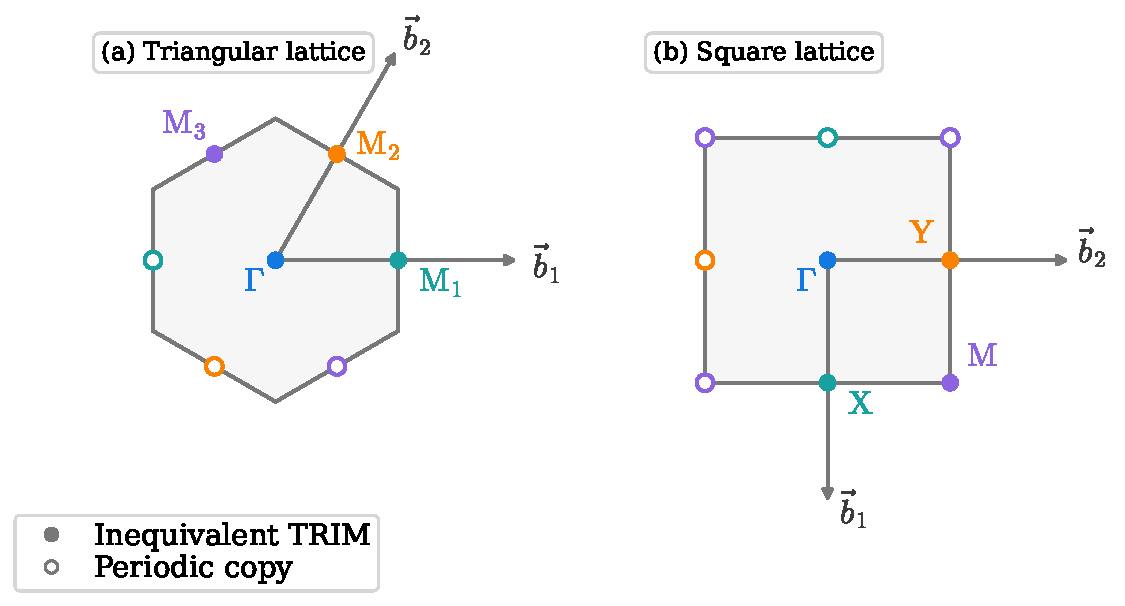
\includegraphics[width=0.95\textwidth]{figures_ch4/4.2_trim.pdf}
\caption{Time-reversal invariant momenta in schematic two-dimensional Brillouin zones.
(a) A triangular lattice has $\Gamma$ and three inequivalent $\mathrm{M}$ points in its hexagonal Brillouin zone.
(b) A square lattice has $\Gamma$, $\mathrm{X}$, $\mathrm{Y}$, and $\mathrm{M}$ as four representatives.
Filled points identify one representative of each TRIM, while open points mark periodic copies on the boundary.
The points satisfy equation~\eqref{four_trim_two_dimensions_topology}, with representatives translated by reciprocal-lattice vectors where necessary.
The diagrams indicate momentum locations only; they contain no calculated parity eigenvalues.}
\label{fig:four_trim_two_dimensions}
\end{figure}

The boundary copies in figure~\ref{fig:four_trim_two_dimensions} do not provide additional independent factors in the parity product.
They represent the same crystal momenta after a reciprocal-lattice translation.
Likewise, the corners conventionally denoted by $\mathrm{K}$ in the hexagonal Brillouin zone are not TRIM:
time reversal exchanges the two inequivalent corners rather than returning either one to itself.

\subsection{Inversion and the parity of a Kramers pair}

We next introduce the inversion operator $\hat{\mathcal{I}}$.
We choose the real-space origin at an inversion centre,
so inversion changes $\vec{r}$ to $-\vec{r}$ and leaves spin unchanged.
Its action on a Bloch state can be expressed through a position projection:

\begin{equation}
    \bra{\vec{r}\,}\hat{\mathcal{I}}\ket{\psi_{n\vec{k}}}
    =\braket{-\vec{r}\,|\psi_{n\vec{k}}}
\label{inversion_position_projection_topology}
\end{equation}

here, the projection leaves the spin components implicit.
For an inversion-symmetric hamiltonian, we have:

\begin{equation}
\left\{\begin{aligned}
    \hat{\mathcal{I}}^2&=\hat{I} \\
    \hat{\mathcal{I}}\hat{h}(\vec{k})\hat{\mathcal{I}}^{-1}
    &=\hat{h}(-\vec{k}) \\
    [\hat{\mathcal{I}},\hat{\Theta}]&=0
\end{aligned}\right.
\label{inversion_symmetry_relations_topology}
\end{equation}

Both inversion and time reversal reverse the crystal momentum.
Their combination consequently leaves $\vec{k}$ unchanged.
Since $(\hat{\mathcal{I}}\hat{\Theta})^2=-\hat{I}$,
the same antiunitary argument used above gives a twofold degeneracy at every $\vec{k}$
when both symmetries are present.
At the TRIM, we can additionally choose the states to diagonalize inversion.

At a TRIM, inversion maps a Bloch state to the same crystal momentum modulo a reciprocal-lattice vector.
We can therefore choose the full Bloch states with definite inversion parity and write:

\begin{equation}
    \hat{\mathcal{I}}\ket{\psi_{n\vec{\Lambda}_i}}
    =\xi_n(\vec{\Lambda}_i)\ket{\psi_{n\vec{\Lambda}_i}},
    \qquad \xi_n(\vec{\Lambda}_i)=\pm1
\label{parity_eigenvalue_topology}
\end{equation}

here, $\xi_n$ is the parity eigenvalue.
The values $+1$ and $-1$ describe even and odd inversion parity, respectively.
Within a degenerate eigenspace, the states can be chosen as simultaneous energy and parity eigenstates.
An arbitrary numerical basis of that eigenspace need not already have this form.

We now apply inversion to the time-reversed partner.
Since inversion commutes with time reversal and $\xi_n$ is real, we obtain:

\begin{equation}
\begin{aligned}
    \hat{\mathcal{I}}\hat{\Theta}\ket{\psi_{n\vec{\Lambda}_i}}
    &=\hat{\Theta}\hat{\mathcal{I}}\ket{\psi_{n\vec{\Lambda}_i}} \\
    &=\xi_n(\vec{\Lambda}_i)
    \hat{\Theta}\ket{\psi_{n\vec{\Lambda}_i}}
\end{aligned}
\label{equal_parity_kramers_pair_topology}
\end{equation}

Therefore, the two states of a Kramers pair have the same parity.
This result determines how parity eigenvalues must be counted in the topological criterion.
Counting both states separately would square every pair contribution and remove the sign information that we need.

\newpage
\section{From parity eigenvalues to the two-dimensional \texorpdfstring{$Z_2$}{Z2} index}
\label{sec:fu_kane_criterion_topology}

% opening paragraph
We have now established the selected band subspace, its phase freedom, and the pairing imposed by symmetry.
The remaining question is whether this subspace can change its topological character continuously while preserving time-reversal symmetry and its separation from the excluded bands.
The two-dimensional $Z_2$ index distinguishes two possibilities for this spinful band problem~\cite{kane2005z2}.
Inversion symmetry then allows us to evaluate that index using the parity information at the four TRIM.
Time reversal is the symmetry that protects this $Z_2$ classification;
inversion supplies the simpler route for evaluating it.
If inversion is removed while time reversal and the band separation are preserved,
the index remains unchanged, although the parity criterion is no longer available.

\subsection{The two topological classes}

We first consider a continuous change of the hamiltonian,
such as a change in bond geometry or in the strength of spin-orbit coupling.
As long as the selected subspace remains isolated and time-reversal symmetry is preserved,
its $Z_2$ index cannot change.
We denote the two possible values by $\nu=0$ and $\nu=1$.
The former is trivial with respect to this index, while the latter is non-trivial.

In terms of electronic states, the distinction concerns whether a globally smooth basis can be chosen
with a consistent time-reversal pairing and the reciprocal-lattice identification introduced above.
For $\nu=1$, this time-reversal-compatible choice is obstructed.
This does not mean that the projector itself is discontinuous,
or that all smooth choices of basis are forbidden.
The constraint comes from requiring the basis to satisfy the time-reversal pairing as well as the global continuity conditions~\cite{kane2005z2}.

For an insulating filling, this distinction has a physical consequence at an interface with a topologically trivial insulator.
Within the non-interacting description and with time-reversal symmetry preserved at the boundary,
the non-trivial phase supports an odd number of Kramers pairs of edge modes connecting the bulk bands.
This explains why a bulk wave-function property is of physical interest.
For a metallic filling, however, the same interpretation cannot be inferred from a parity sign alone,
because bulk states can remain at the Fermi level.

\subsection{The Fu--Kane parity product}

We now use inversion symmetry to evaluate $\nu$.
For each TRIM $\vec{\Lambda}_i$, we first multiply one parity eigenvalue from each of the $N_\mathrm{p}$ Kramers pairs in the selected subspace:

\begin{equation}
    \delta_i
    \coloneqq\prod_{m=1}^{N_\mathrm{p}}\xi_{2m}(\vec{\Lambda}_i)
\label{parity_product_at_trim_topology}
\end{equation}

here, the indices $(2m-1,2m)$ label the members of a Kramers pair,
chosen so that both states have the same parity according to equation~\eqref{equal_parity_kramers_pair_topology}.
The subspace contains $2N_\mathrm{p}$ spinor states, but the product contains $N_\mathrm{p}$ factors.
The use of $2m$ selects one representative from each pair.

The Fu--Kane criterion relates these four products to the two-dimensional index~\cite{fu2007topological}:

\begin{equation}
\left\{\begin{aligned}
    (-1)^\nu&=\prod_{i=1}^{4}\delta_i \\
    \nu&=
    \begin{cases}
        0, & \prod_{i=1}^{4}\delta_i=+1 \\
        1, & \prod_{i=1}^{4}\delta_i=-1
    \end{cases}
\end{aligned}\right.
\label{fu_kane_index_topology}
\end{equation}

This criterion supplies the connection between inversion eigenvalues and the global time-reversal classification.
The equality of the two parities in each pair explains the counting in equation~\eqref{parity_product_at_trim_topology};
the identification of the four-point product with $(-1)^\nu$ is the additional topological result.
It is not obtained by counting degeneracies alone.

The result also explains why the parity of a single state or the ordering at one momentum is insufficient.
Every selected Kramers pair contributes at each of the four TRIM.
If one selected pair exchanges with an excluded pair of opposite parity at a TRIM,
that exchange changes the local product when the gap reopens.
An odd number of such sign changes changes the global product,
whereas an even number leaves it unchanged.
The exchange must pass through a closure of the separation between the two subspaces.
An exchange wholly within the selected subspace instead preserves the product because neither pair leaves the count.

\subsection{Using additional crystal symmetry}

For the hexagonal Brillouin zone in figure~\ref{fig:four_trim_two_dimensions}(a),
the general product is:

\begin{equation}
    (-1)^\nu
    =\delta_\Gamma\delta_{\mathrm{M}_1}
    \delta_{\mathrm{M}_2}\delta_{\mathrm{M}_3}
\label{hexagonal_trim_product_topology}
\end{equation}

If crystal symmetry relates the three $\mathrm{M}$ points with equal parity products in the chosen inversion convention,
we can set $\delta_{\mathrm{M}_1}=\delta_{\mathrm{M}_2}=\delta_{\mathrm{M}_3}=\delta_\mathrm{M}$.
The product then reduces to $\delta_\Gamma(\delta_\mathrm{M})^3=\delta_\Gamma\delta_\mathrm{M}$.

For the square Brillouin zone in figure~\ref{fig:four_trim_two_dimensions}(b),
we similarly retain all four representatives first:

\begin{equation}
    (-1)^\nu
    =\delta_\Gamma\delta_\mathrm{X}\delta_\mathrm{Y}\delta_\mathrm{M}
\label{square_trim_product_topology}
\end{equation}

If the actual structure relates $\mathrm{X}$ and $\mathrm{Y}$ with equal parity products,
then $\delta_\mathrm{X}\delta_\mathrm{Y}=(\delta_\mathrm{X})^2=1$,
and the same reduced expression follows.
The equality of the final expressions does not make the two Brillouin zones equivalent.
It results from different symmetry relations among their four TRIM.

These reductions require the symmetry of the calculated structure and a consistent inversion centre.
The appearance of a high-symmetry path alone does not establish the equality of the omitted products.
Keeping all four factors until their relation has been checked makes the reduction explicit
and connects the numerical parity data to the general criterion in equation~\eqref{fu_kane_index_topology}.

\newpage
\section{From the parity criterion to the calculation}
\label{sec:interpreting_topology_calculation}

% opening paragraph
The previous section connected the parity eigenvalues to the $Z_2$ index.
We now return to the first-principles setting introduced in subsection~\ref{subsec:method_topology}.
The calculation must supply the same ingredients used in that connection:
a specified spinor hamiltonian, the relevant symmetries, an isolated band subspace, and the parity of its Kramers pairs.
The interpretation then follows from the relation between that subspace and the Fermi level.

\subsection{Identifying the states used in the product}

We first determine the crystal symmetry and the reciprocal lattice of the relaxed structure.
These determine the inversion operation and the four TRIM.
For the spinful classification used here, the electronic states are calculated with spin-orbit coupling,
and the reference state must preserve time-reversal symmetry.
The small atomic number of an element does not justify omitting spin-orbit coupling from this step:
a small coupling may still affect a band crossing or a small separation relevant to the selected subspace.

We then select the fixed number $2N_\mathrm{p}$ of bands and examine
$\Delta_\mathrm{dir}(\vec{k})$ from equation~\eqref{minimum_direct_gap_topology}.
For an insulator, this selection can coincide with all the occupied spinor bands.
For a metal, the number of states below $E_\mathrm{F}$ can change with $\vec{k}$,
so the phrase ``occupied bands'' alone does not identify the subspace.
Numerical smearing of the occupations also does not define a fixed-rank projector.
The band count must instead refer to the selected spectral subspace at every wave vector.

The direct separation has to be checked over the two-dimensional Brillouin zone.
A band plot along a high-symmetry path samples only part of that zone.
In practice, a converged two-dimensional sampling, with refinement near the smallest separations,
provides evidence for the gap condition within the numerical accuracy of the calculation.
If interpolation is used, its accuracy near those separations must be checked against direct calculations.
A near-zero separation requires particular care because an unresolved touching point changes whether the chosen spectral subspace is isolated.

At each TRIM, the parity eigenvalues can be obtained from the symmetry representation of the spinor states.
The \texttt{irvsp} method used in chapter~\ref{cha:project_beryllene}
extracts such symmetry information from VASP wave functions~\cite{gao2021irvsp}.
For a degenerate group, the inversion representation must be resolved within that group,
so an arbitrary numerical mixture is not mistaken for a parity eigenstate.
We then identify complete Kramers pairs, count one parity from each pair,
and evaluate the four factors in equation~\eqref{parity_product_at_trim_topology}.

\subsection{Interpreting the resulting index}

Once the subspace and symmetries have been established, the parity product assigns $\nu$ to that specified subspace.
We next compare its energy range with the physical Fermi level.
If equation~\eqref{insulating_fermi_level_topology} holds,
the subspace is the occupied space of a band insulator,
and $\nu=1$ identifies the non-trivial two-dimensional time-reversal phase within the band description.

If the direct separation remains positive but the indirect separation is negative,
we can still discuss the topology of the isolated lower-band subspace.
The actual Fermi-level state nevertheless remains metallic at an overlapping filling.
Thus the topological index and the metallic character describe different aspects of the same band structure,
as illustrated in figure~\ref{fig:band_subspace_and_insulating_gap}(b).
If the selected and excluded bands touch,
the isolation condition used throughout this chapter is absent,
and this fixed-rank spectral-subspace argument cannot be applied without further justification.

This distinction also clarifies the relation to the optical analysis.
The independent-particle response in equation~\eqref{independent_particle_imaginary_dielectric_tensor}
uses actual occupation differences, transition matrix elements, and transition energies.
The parity criterion instead characterizes the connection of a specified band subspace over the Brillouin zone.
The optical spectrum therefore resolves the allowed electronic excitations,
while the parity product classifies the symmetry-constrained connection of the selected states.
The Fermi-level condition determines whether this classification describes an insulating phase.

At this stage, we have connected the Bloch-state description to the symmetry analysis used in the beryllene project.
Chapter~\ref{cha:fundamentals_a} supplies the electronic structure,
chapter~\ref{cha:fundamentals_b} connects that structure to its linear optical response,
and the present chapter explains the band-subspace and symmetry conditions required for the topological classification.
The material-specific band selection, gap evidence, and parity eigenvalues belong to the corresponding research calculation.
These quantities determine which of the interpretations developed here applies to each system.
